\documentclass[letterpaper]{scrartcl}
\usepackage{lmodern}
\usepackage{amssymb,amsmath}
\usepackage{ifxetex,ifluatex}
\usepackage{fixltx2e} % provides \textsubscript
\ifnum 0\ifxetex 1\fi\ifluatex 1\fi=0 % if pdftex
  \usepackage[T1]{fontenc}
  \usepackage[utf8]{inputenc}
\else % if luatex or xelatex
  \ifxetex
    \usepackage{mathspec}
    \usepackage{xltxtra,xunicode}
  \else
    \usepackage{fontspec}
  \fi
  \defaultfontfeatures{Mapping=tex-text,Scale=MatchLowercase}
  \newcommand{\euro}{€}
\fi
% use upquote if available, for straight quotes in verbatim environments
\IfFileExists{upquote.sty}{\usepackage{upquote}}{}
% use microtype if available
\IfFileExists{microtype.sty}{%
\usepackage{microtype}
\UseMicrotypeSet[protrusion]{basicmath} % disable protrusion for tt fonts
}{}
\usepackage[margin=1in]{geometry}
\usepackage{graphicx}
\makeatletter
\def\maxwidth{\ifdim\Gin@nat@width>\linewidth\linewidth\else\Gin@nat@width\fi}
\def\maxheight{\ifdim\Gin@nat@height>\textheight\textheight\else\Gin@nat@height\fi}
\makeatother
% Scale images if necessary, so that they will not overflow the page
% margins by default, and it is still possible to overwrite the defaults
% using explicit options in \includegraphics[width, height, ...]{}
\setkeys{Gin}{width=\maxwidth,height=\maxheight,keepaspectratio}
\ifxetex
  \usepackage[setpagesize=false, % page size defined by xetex
              unicode=false, % unicode breaks when used with xetex
              xetex]{hyperref}
\else
  \usepackage[unicode=true]{hyperref}
\fi
\hypersetup{breaklinks=true,
            bookmarks=true,
            pdfauthor={},
            pdftitle={Supplemental Methods for LD filtering},
            colorlinks=true,
            citecolor=blue,
            urlcolor=blue,
            linkcolor=magenta,
            pdfborder={0 0 0}}
\urlstyle{same}  % don't use monospace font for urls
\setlength{\parindent}{0pt}
\setlength{\parskip}{6pt plus 2pt minus 1pt}
\setlength{\emergencystretch}{3em}  % prevent overfull lines
\setcounter{secnumdepth}{5}

\title{Supplemental Methods for LD filtering}
\date{}
\usepackage{fontspec}
\setmainfont{Linux Libertine O}

% blockquote


\begin{document}
\maketitle

{
\hypersetup{linkcolor=black}
\setcounter{tocdepth}{3}
\tableofcontents
}
\section{LD-based filtering of
SNP-pairs}\label{ld-based-filtering-of-snp-pairs}

The LD values of SNP-pairs were compared after binning SNP-pairs by base
pair separation to control for unknown rates of recombination in
\emph{G. f. fuscipes}. Bin length was set at 50 bp with the lower bound
inclusive and higher bound exclusive. In other words the bins were
defined as \([i, i + 49)\) where
\(i \in \{1,1(50),2(50),3(50) ... n(50)\}\) and \(n\) is a positive
integer.

To identify SNP-pairs for further investigation in an arbitrary set of
binned SNP-pairs, we needed to assign probabilities to each SNP-pair in
the bin. The distributions of binned SNP-pairs are bounded by 0 and 1
and do not appear to be Normal in shape. Additionally, in many cases,
the data appear to exhibit peaks at both the lower and upper \(r^2\)
range. This suggested that the data may be modeled well using the
probability density function (PDF) of the Beta distribution:

\[f(x;\alpha,\beta) = \frac{x^{\alpha-1}(1-x)^{\beta-1}} {\mathrm{B}(\alpha,\beta)}\]

with shape parameters \(\alpha\) and \(\beta\) and where \(x\)
represents an observed value generated by the distribution and
\(\mathrm{B}()\) is the Beta function.

The Beta's cumulative distribution function (CDF):

\[F(x;\alpha,\beta) = \frac{\mathrm{B}(x;\alpha,\beta)}{\mathrm{B}(\alpha,\beta)} \]

can be used to describe the probability that a binned SNP-pair will be
observed to have an \(r^2 \le x\). It follows that \(1-\mathrm{CDF}\)
represents the probability of observing a more extreme value.

For each set of binned \(r^2\) values, the SNP-pairs deemed worthy of
further investigation were defined as those where
\(1-\mathrm{CDF} \le 0.01\) after Benjamini-Hochberg (BH) correction for
multiple testing {[}1{]}.

\subsection{Scaling of binned \(r^2\)
distributions}\label{scaling-of-binned-r2-distributions}

The Beta distribution is bounded on the non-inclusive interval between 0
and 1. However, there are data in each bin that may have been assigned
values of exactly 0 or 1. It is likely that these values are not truly 0
or 1 in the discrete binary sense that a coin-flip is \emph{either}
heads or tails. Therefore, the all data for each bin were scaled
according to the following scheme

\[((x_i - 0.5)\cdot \theta) + 0.5\]

in order to symmetrically shrink the distribution of values to fit
within the open interval \((0,1)\). In the scheme above, let \(x_i\)
stand for the \(r^2\) of each SNP-pair in an arbitrary bin set and
\(\theta\) stand for the scaling factor. The relevant results in this
paper used \(\theta = 0.999\).

\subsection{Bayesian parameter estimation using the binned \(r^2\)
distributions}\label{bayesian-parameter-estimation-using-the-binned-r2-distributions}

In order to use the CDF of the Beta distribution to assign significances
to each observed SNP-pair in a bin, it is necessary to learn the
distribution parameters (\(\alpha\) and \(\beta\)) for each bin given
the specific data in each bin. For this we used custom python code that
made heavy use of the following third-party data analysis modules:
Pandas {[}2{]}, NumPy {[}3{]}, SciPy {[}4{]}, pyMC {[}5{]}, and
StatsModels {[}6{]}.

We used pyMC to build the model of the Beta distribution and use it to
exploit the bin-specific data to estimate the bin-specific values for
the \(\alpha\) and \(\beta\) parameters of the model {[}Figure
fig\_betamod{]}. The values of \(\alpha\) and \(\beta\) were modeled
with separate Uniform prior distributions from 0.01 to 10. This model
topology was used to create pyMC ``model'' objects and initialized with
the \(r^2\) data from each bin. The parameters of each Beta distribution
were then estimated by \emph{maximum a posteriori} (MAP) and used to
calculate the \(1-\mathrm{CDF}\) for each SNP-pair in each bin
{[}3,4{]}. The \(1-\mathrm{CDF}\) values were then BH corrected by bin
and filtered with a threshold of \((1-CDF)_{BH} \le 0.01\) using
statsmodels {[}1{]}.

\section{Code availability}\label{code-availability}

The code used to run this and other parts of the analyses described in
this manuscript may be found on github at the following project address.

\url{https://github.com/CacconeLabYale/gloria_soria_ddRAD_2015}

\hyperdef{}{figux5fbetamod}{}
\begin{figure}[htbp]
\centering
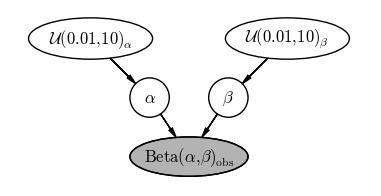
\includegraphics{../figures/bin_MAP_model.png}
\caption{\textbf{{[}fig\_betamod{]}Network representation of the LD Beta
model:} Ovals represent modeled probability distributions. Circles
represent learned parameters. Grey shading indicates use of observed
data. \label{fig_betamod}}
\end{figure}

\newpage

\section*{Bibliography}\label{bibliography}
\addcontentsline{toc}{section}{Bibliography}

1. Benjamini Y, Hochberg Y. Controlling the False Discovery Rate: A
Practical and Powerful Approach to Multiple Testing. Journal of the
Royal Statistical Society Series B (Methodological). Wiley for the Royal
Statistical Society; 1995;57: pp. 289--300. Available:
\url{http://www.jstor.org/stable/2346101}

2. McKinney W. Data Structures for Statistical Computing in Python. In:
Walt S van der, Millman J, editors. Proceedings of the 9th python in
science conference. 2010. pp. 51--56.

3. {Van Der Walt} S, Colbert SC, Varoquaux G. The NumPy array: A
structure for efficient numerical computation. Computing in Science and
Engineering. 2011;13: 22--30.
doi:\href{http://dx.doi.org/10.1109/MCSE.2011.37}{10.1109/MCSE.2011.37}

4. Jones E, Oliphant T, Peterson P, Others. SciPy: Open source
scientific tools for Python {[}Internet{]}. 2001. Available:
\url{http://www.scipy.org/}

5. Patil A, Huard D, Fonnesbeck CJ. PyMC: Bayesian Stochastic Modelling
in Python. Journal of statistical software. 2010;35: 1--81. Available:
\url{http://www.pubmedcentral.nih.gov/articlerender.fcgi?artid=3097064/\&tool=pmcentrez/\&rendertype=abstract}

6. Statsmodels-development-team. StatsModels: Statistics in Python
(v0.6.1) {[}Internet{]}. Available:
\url{http://statsmodels.sourceforge.net/stable/}

\end{document}
